\documentclass[12pt,a4paper]{article}
\usepackage[utf8]{vietnam}
\usepackage{amsmath}
\usepackage{amsfonts}
\usepackage{amssymb}
\usepackage{graphicx}
\usepackage[left=2cm,right=2cm,top=2cm,bottom=2cm]{geometry}
\usepackage{fancyhdr}
\pagestyle{fancy}
\fancyhead{} % clear all header fields
\fancyhead[L]{
 \begin{tabular}{rl}
    \begin{picture}(25,15)(0,0)
    \put(0,-8){
\includegraphics[width=8mm, height=8mm]{hcmut.png}}
   \end{picture}&
	\begin{tabular}{l}
		\textbf{\bf \ttfamily Trường Đại Học Bách Khoa Tp.Hồ Chí Minh}\\
		\textbf{\bf \ttfamily Khoa Khoa Học và Kỹ Thuật Máy Tính}
	\end{tabular} 	
 \end{tabular}
}
\fancyhead[R]{
	\begin{tabular}{l}
		\tiny \bf \\
		\tiny \bf 
	\end{tabular}  }


\begin{document}
\begin{titlepage}
\begin{center}
\large\textbf{ĐẠI HỌC QUỐC GIA TP. HỒ CHÍ MINH\\
TRƯỜNG ĐẠI HỌC BÁCH KHOA\\
KHOA KHOA HỌC VÀ KỸ THUẬT MÁY TÍNH}\\
\vspace{1.5cm}

\includegraphics[scale=0.09]{hcmut.png} \\
\vspace{1.5cm}
\LARGE{\textbf{MẠNG MÁY TÍNH}}\\
\vspace{1.7cm}
\rule{15cm}{0.06cm}
\begin{flushleft}
\hspace{1cm}
\Large\textbf{Báo cáo Bài tập lớn 1}
\end{flushleft}
\LARGE\textbf{STREAMING VIDEO}
\rule{15cm}{0.06cm}
\end{center}
\vspace{1 cm}
\begin{table}[h]
\begin{tabular}{rrll}
\hspace{5 cm} & GVHD: & Th.S Nguyễn Hồng Nam\\
& SV thực hiện: & Nguyễn Phi Thông & 1814205 \\
& & Nguyễn Văn Thuần & 1814220 \\
& & Lộc Quốc Huy & 1812369 \\
& & Lê Văn Thi & 1613298 \\
\end{tabular}
\end{table}
\vspace{1.5cm}
\begin{center}
{\footnotesize Tp. Hồ Chí Minh, Tháng 11/2020}
\end{center}
\end{titlepage}
\tableofcontents
\newpage
\section{Phân tích yêu cầu}
\subsection{Mục tiêu}
Mục tiêu của bài tập lớn là chúng ta sẽ hiện thực streaming video server và client sử dụng Real-Time Streaming Protocol (RTSP) để giao tiếp và Real-Time Tranfer Protocol (RTP) để gửi dữ liệu.
\subsection{Yêu cầu}
\subsubsection{Client}
Hiện thực RTSP protocol. Chúng ta cần hoàn thành các function mà được gọi khi người dùng click vào các button trên giao diện người dùng. Khi client bắt đầu, RTSP socket sẽ được mở đến server và sử dụng socket này cho việc gửi các yêu cầu RTSP. Các button: 
\begin{itemize}
\item \textbf{SETUP} \\Command này sẽ thiết lập các session và tham số truyền tải.
\item \textbf{PLAY} \\Command này sẽ playback cho client.
\item \textbf{PAUSE} \\Command này sẽ tạm dừng việc playback.
\item \textbf{TEARDOWN} \\Command này sẽ kết thúc session và đóng kết nối.
\end{itemize}
\subsubsection{Server}
Chúng ta tạo ra packet, set các fields trong header của packet và copy payload vào trong packet. Khi server nhận được yêu cầu PLAY từ client, server sẽ đọc một video frame từ file và  tạo ra một đối tượng RtpPacket là RTP-encapsulation của video frame  và gửi frame này  đến client qua UDP sau mỗi 50ms. Để đóng gói, chúng ta sẽ gọi hàm encode của class RtpPacket. Nhiệm vụ của chúng ta là hiện thực cái hàm này theo những bước sau:
\begin{itemize}
\item Set RTP-version (V) = 2.
\item Set padding (P), extension (X), số contributing sources (CC), maker (M), tất cả đều bằng 0.
\item Set payload type (PT) = 26.
\item Set sequence number.
\item Set timestamp.
\item Set sources identifier.  
\end{itemize}
\section{Function description}
\subsection{Client.py}
\begin{itemize}
\item createWidgets: tạo giao diện cho client với 4 button: SETUP, PLAY, PAUSE, TEARDOWN.
\item setupMovie: gửi yêu cầu SETUP đến server.
\item exitClient: gửi yêu cầu TEARDOWN đến server và đóng giao diện người dùng.
\item pauseMovie: gửi yêu cầu PAUSE đến server.
\item playMovie: gửi yêu vầu PLAY đến server.
\item listenRtp: nhận data từ server để decode và update lại số frame.
\item writeFrame: viết các frame nhận được vào 1 file và trả về image file.
\item updateMovie:  update lại image file cũng như video frame trên giao diện.
\item connectToServer: kết nối với server và bắt đầu session RTSP/TCP mới.
\item sendRtspRequest: gửi các request đến server.
\item recvRtspReply: nhận phản hồi từ server. 
\item parseRtspReply: xử lý phản hồi từ server.
\item openRtpPort: mở socket.
\item handler: xử lý event khi người dùng nhấn nút (x) để thoát.
\end{itemize}
\subsection{RtpPacket.py}
\begin{itemize}
\item encode: set các field trong header của RTP packet.
\item decode: tách RTP packet thành header và payload.
\item version: trả về version của RTP.
\item seqNum: trả về sequence number.
\item timestamp: trả về timestamp.
\item payloadType: trả về kiểu của payload.
\item getPayLoad: trả về payload.
\item getPacket: trả về RTP packet.
\end{itemize}
\subsection{ServerWorker.py}
\begin{itemize}
\item run: bắt đầu server.
\item recvRtspRequest: nhận RTSP request từ client.
\item processRtspRequest: xử lý RTSP request từ client.
\item sendRtp: gửi RTP packet qua UDP.
\item makeRtp: RTP-packetize dữ liệu video.
\item replyRtsp: gửi phản hồi RTSP đến 
\end{itemize}
\subsection{VideoStream.py}
\begin{itemize}
\item nextFrame: get frame kế tiếp.
\item frameNbr: trả về fram number.
\end{itemize}
\section{Class diagram}
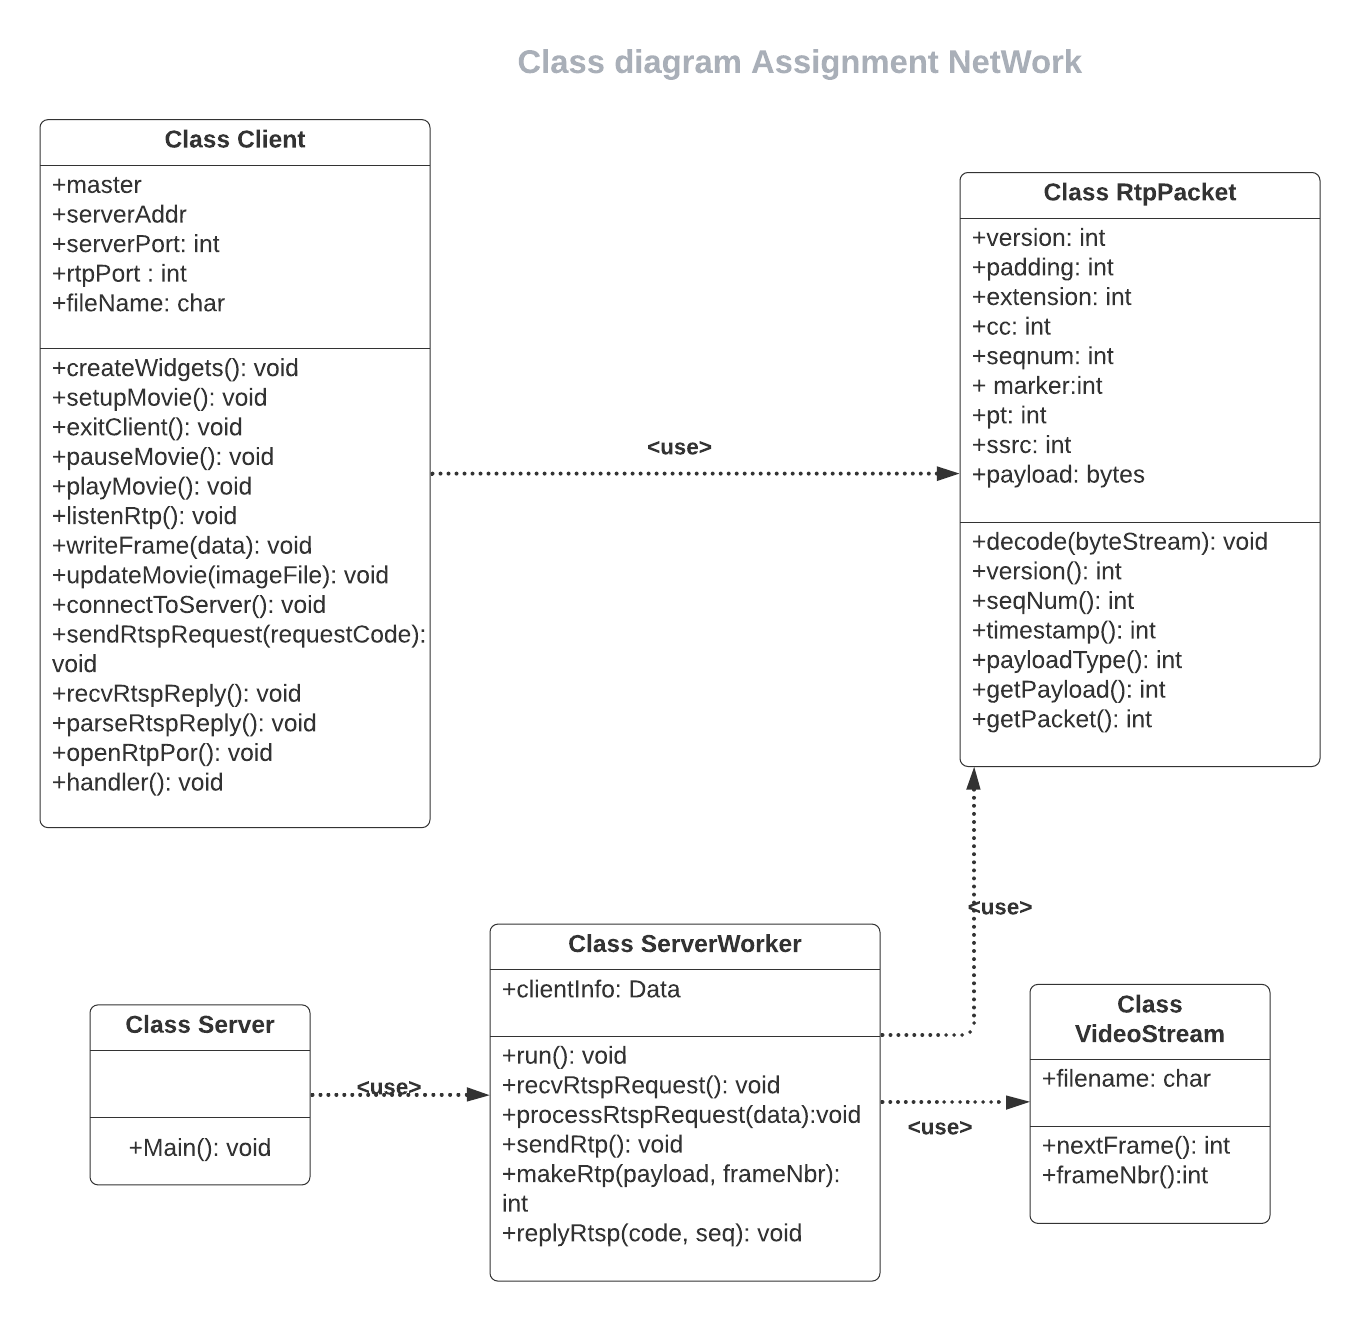
\includegraphics[scale=0.4]{class.png} 
\section{Extend}
\begin{itemize}
    \item Tính toán RTP packet loss rate: Khi cho thực hiện các lệnh chạy trên cùng một mấy cho server và client thì không nhận thấy được sự mất gói trong quá trình phát video. Từ đó, kết luận rằng RTP packet loss rate = 0 trong trường hợp thực hiện chạy các lệnh như trên.
    \item Tính toán video data rate: Sử dụng công thức tính dựa vào kích thước file và thời gian của video. Với kích thước file là 4170 KB và thời gian video đo được là 32 giây thì kết quả thu được là 1.0425 mbps.
\end{itemize}


\section{Hướng dẫn sử dụng}
\begin{enumerate}
\item Bắt đầu server bằng cách chạy file Server.py bằng lệnh sau: \\ \textbf{py Server.py server\_port}\\
Ta nên chọn server\_port lớn hơn 1024, ví dụ ta chọn server\_port = 2000 trong phần hướng dẫn này.
\item Sau đó, ta bắt đầu bên client bằng cách chạy file ClientLauncher.py bằng lệnh sau: \\
\textbf{py ClientLaucher.py server\_host server\_port RTP\_port name\_video} \\
Sau khi chạy lệnh trên, ta sẽ thấy giao diện xuất hiện, và có 4 button \textit{Setup, Play, Pause, TearDown}. Ngoài ra, khung terminal bên trái là bắt đầu server và bên phải là bắt đầu bên client. \\ \\
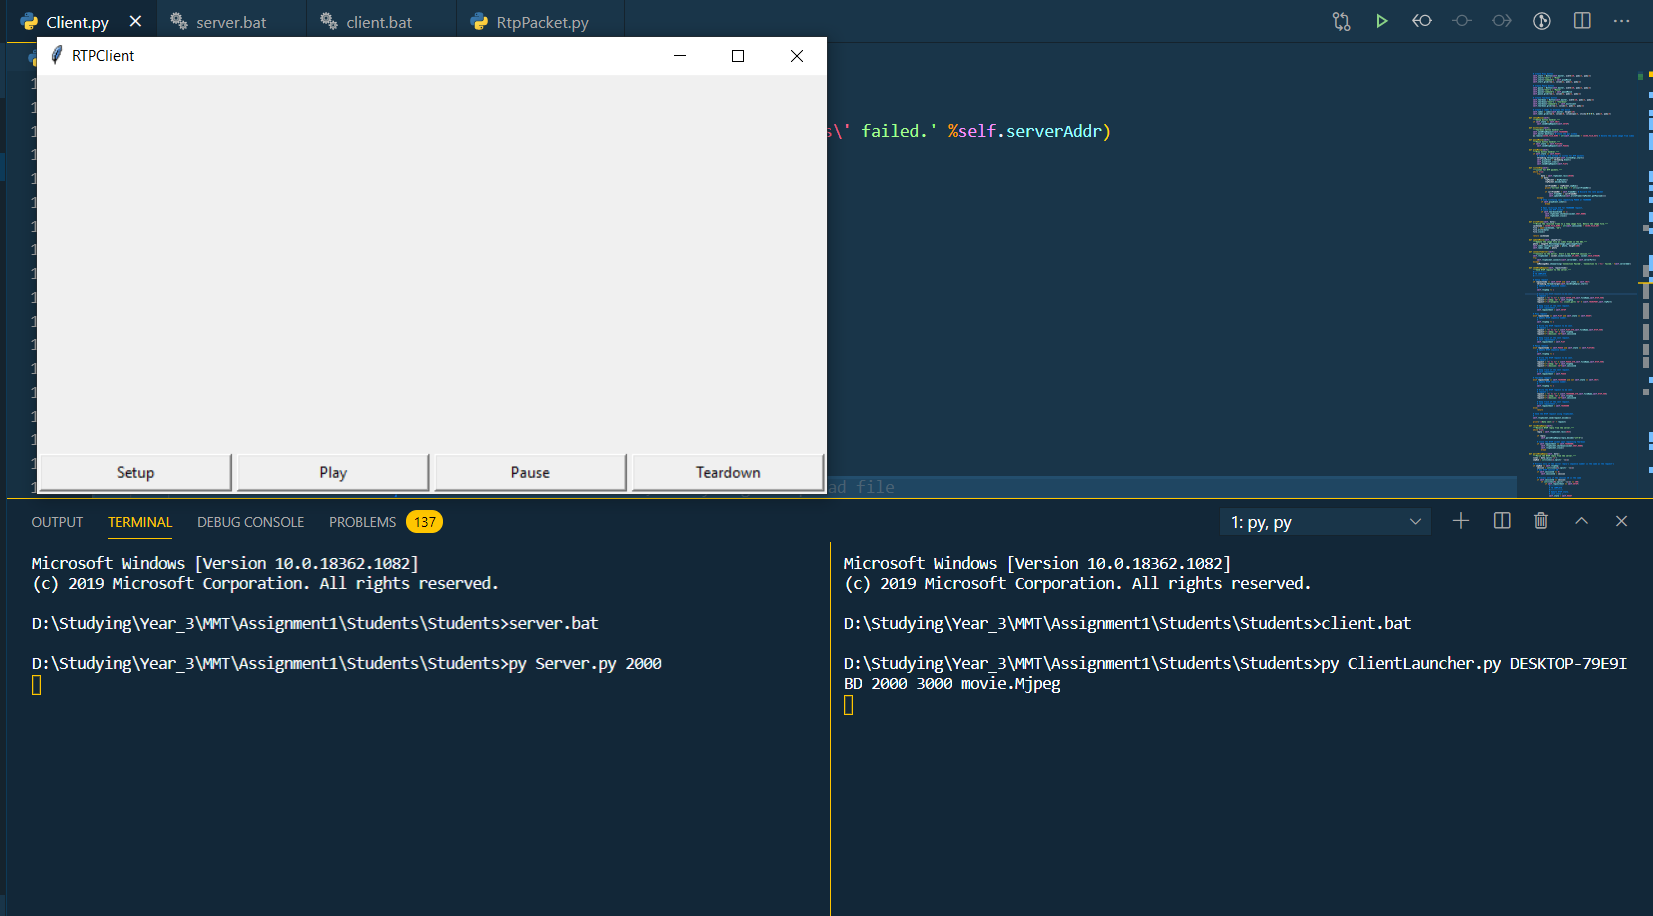
\includegraphics[scale=0.5]{h1.png} 
\item Khi client click vào button \textbf{Setup} \\ \\
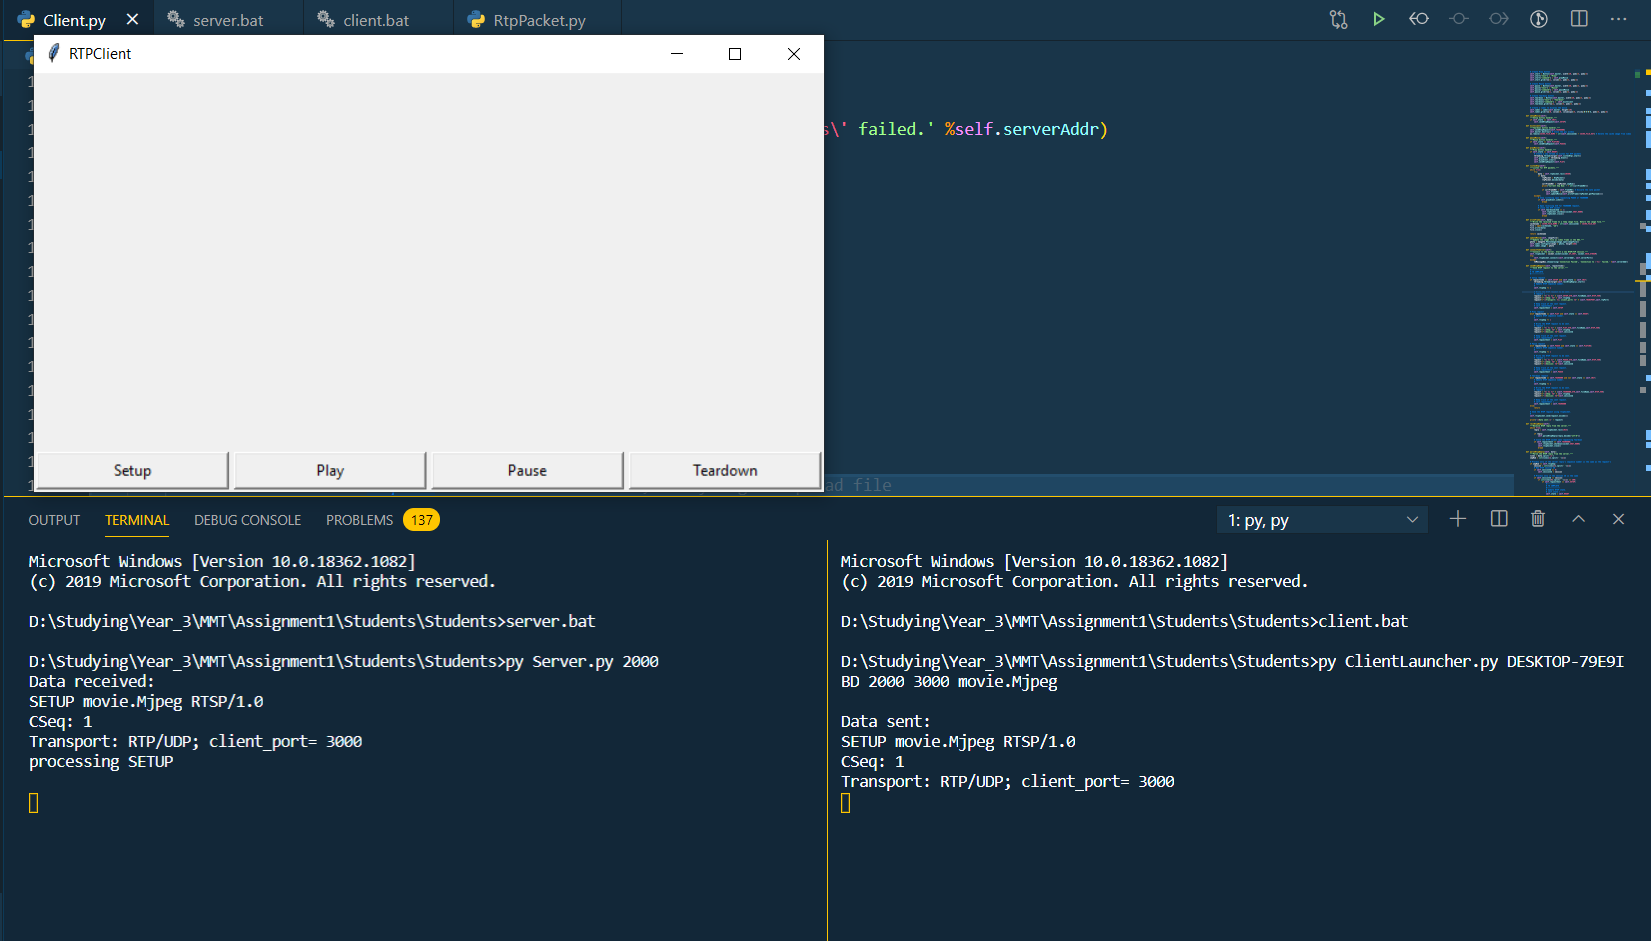
\includegraphics[scale=0.5]{h2.png}  \\
Bên phía client sẽ gửi yêu cầu lên server với data gồm có:
\begin{itemize}
\item Command SETUP
\item Tên video
\item Version RTSP
\item RTSP sequence number
\item Giao thức truyền
\item client\_port
\end{itemize}
Bên phía server sẽ nhận được tất cả data mà client gửi và hiện ra trong terminal cùng với dòng thông báo  \textit{processing SETUP}
\item Khi client click vào button \textbf{Play} \\
\textbf{Server:} \\ \\
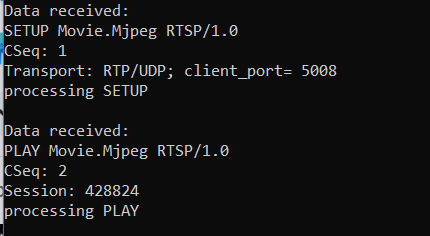
\includegraphics[scale=0.5]{h6.png}  \\
\textbf{Client:} \\ \\
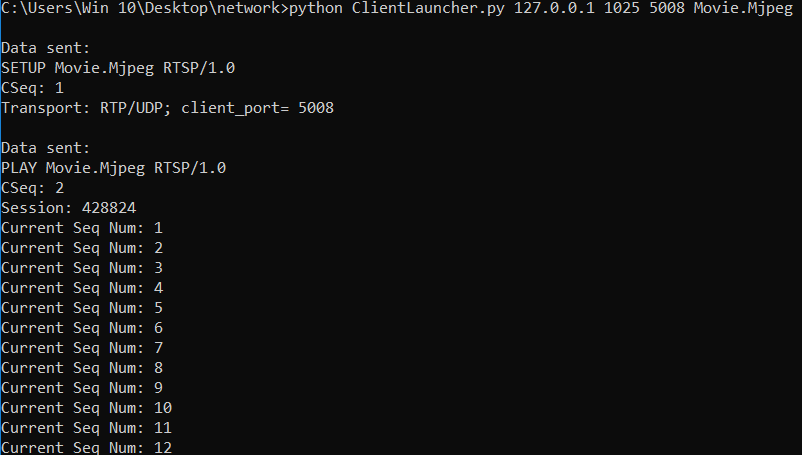
\includegraphics[scale=0.5]{h7.png}  \\
Bên phía client sẽ gửi yêu cầu lên server với data gồm có:
\begin{itemize}
\item Command PLAY  
\item Tên video
\item Version RTSP
\item RTSP sequence number
\item Session 
\item Chuỗi Current Seq Num
\end{itemize}
Bên phía server sẽ nhận được tất cả data mà client gửi và hiện ra trong terminal cùng với dòng thông báo  \textit{processing PLAY}

\item Khi client click vào button \textbf{Pause} \\ \\
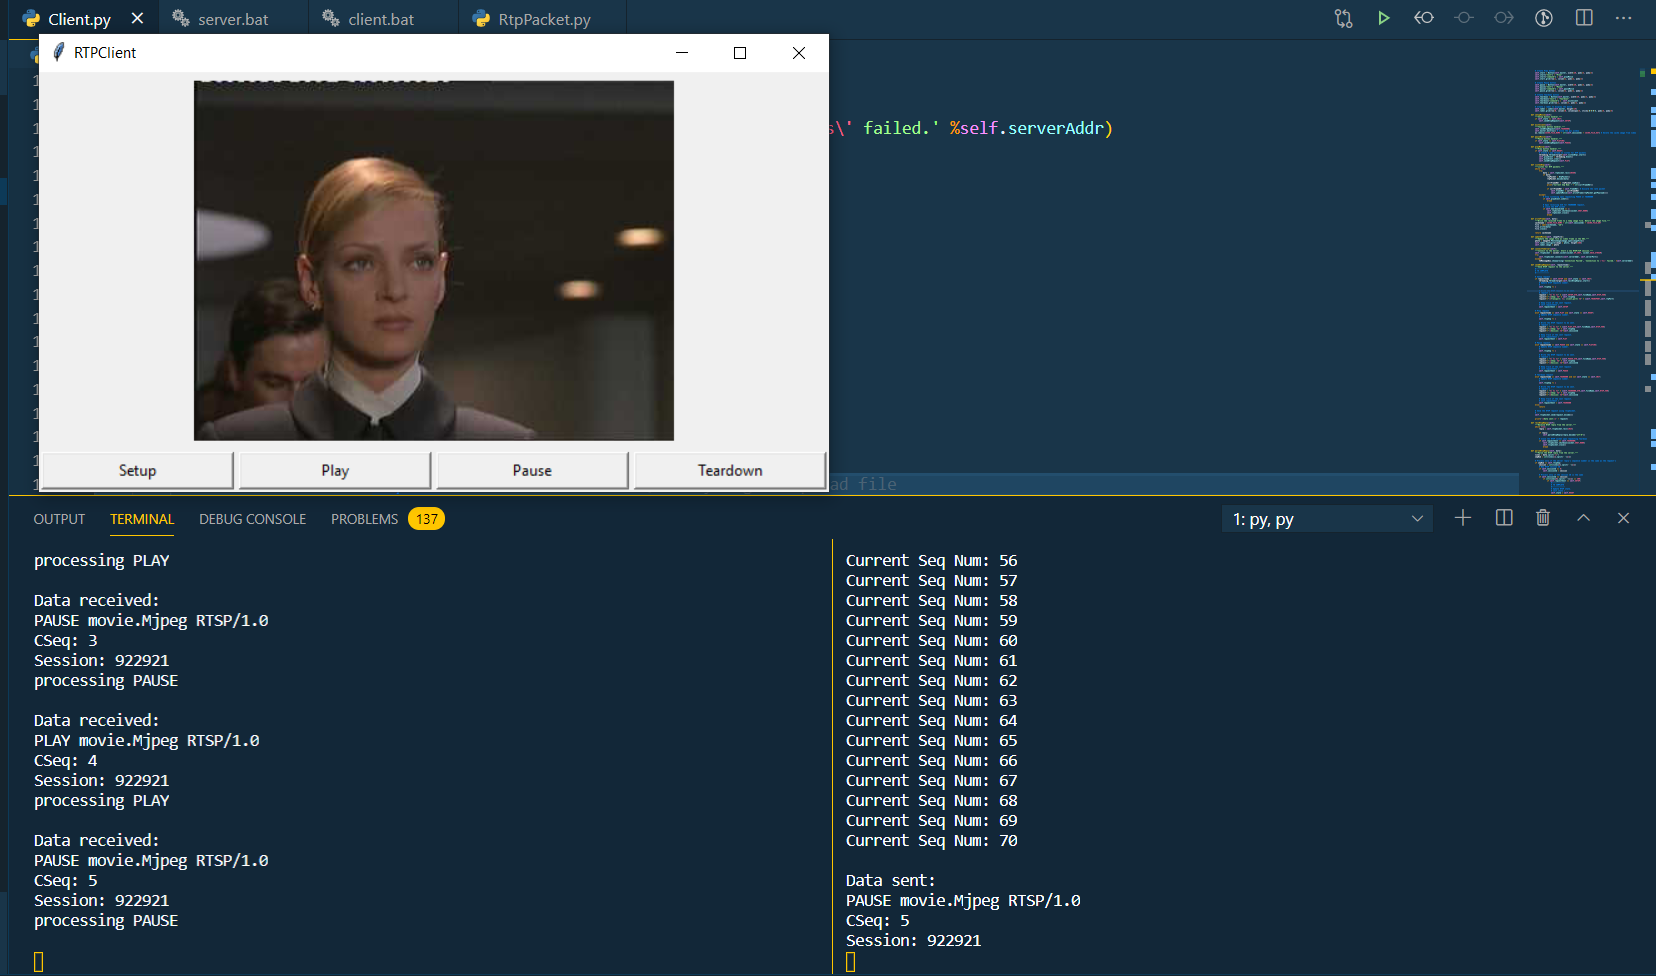
\includegraphics[scale=0.5]{h3.png}  \\ \\
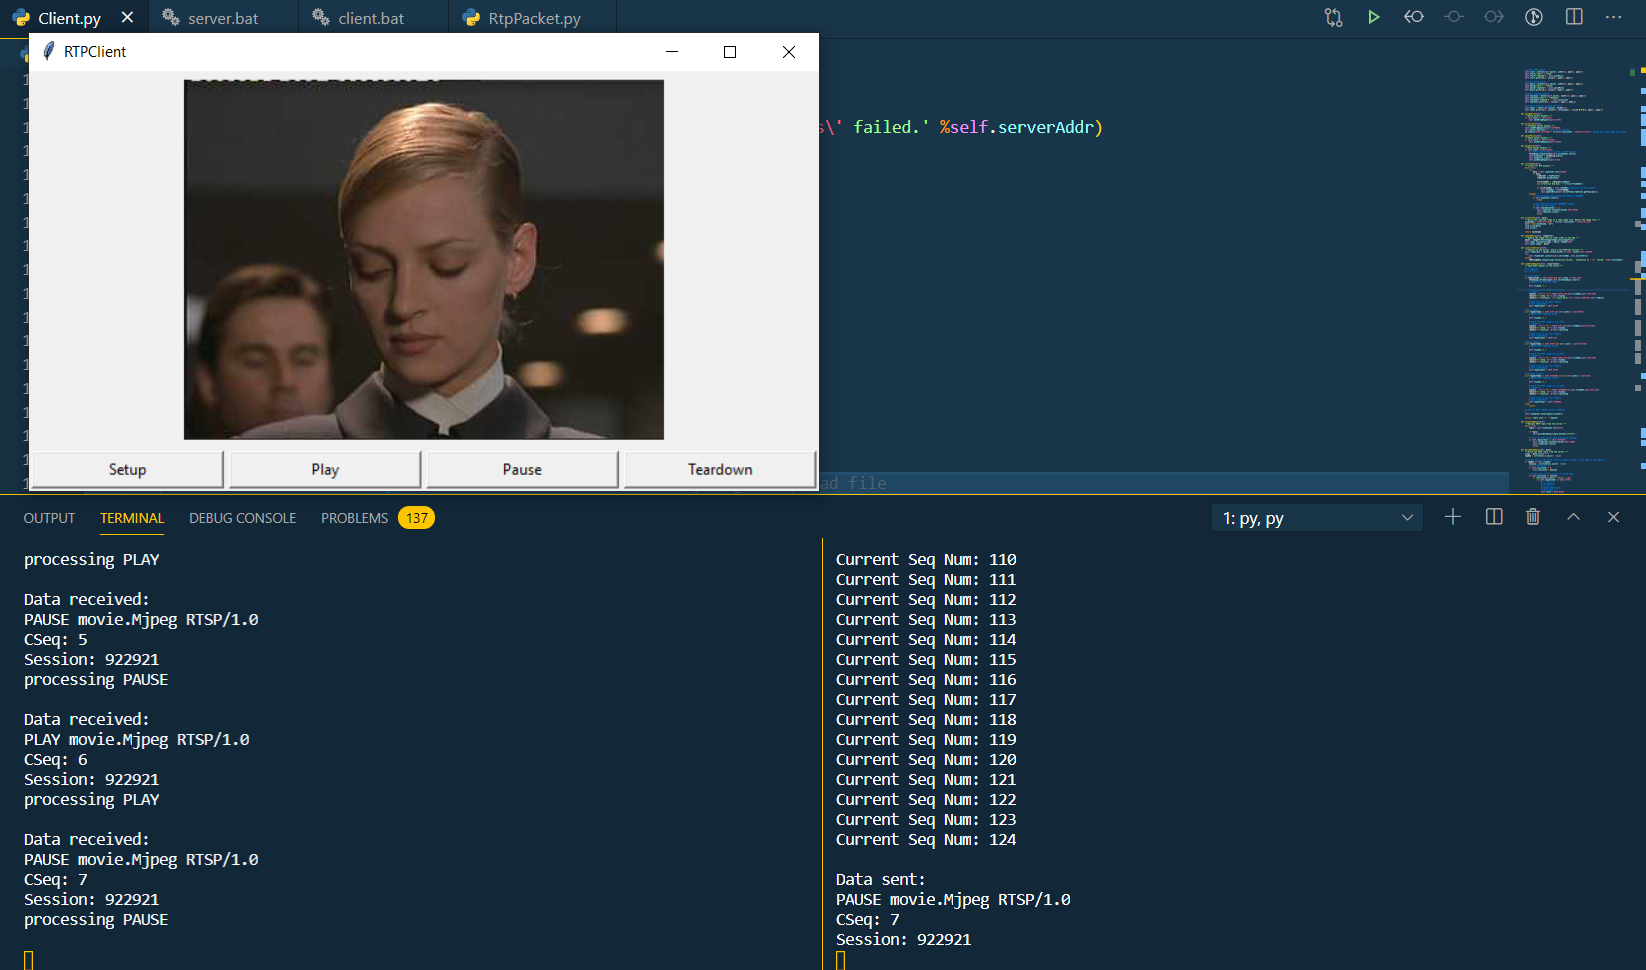
\includegraphics[scale=0.5]{h4.png}  \\ \\
Bên phía client sẽ gửi yêu cầu lên server với data gồm có:
\begin{itemize}
\item Command PAUSE
\item Tên video
\item Version RTSP
\item RTSP sequence number
\item Session 
\end{itemize}
Bên phía server sẽ nhận được tất cả data mà client gửi và hiện ra trong terminal cùng với dòng thông báo  \textit{processing PAUSE}
\item Khi client click vào button \textbf{Teardown} \\ \\
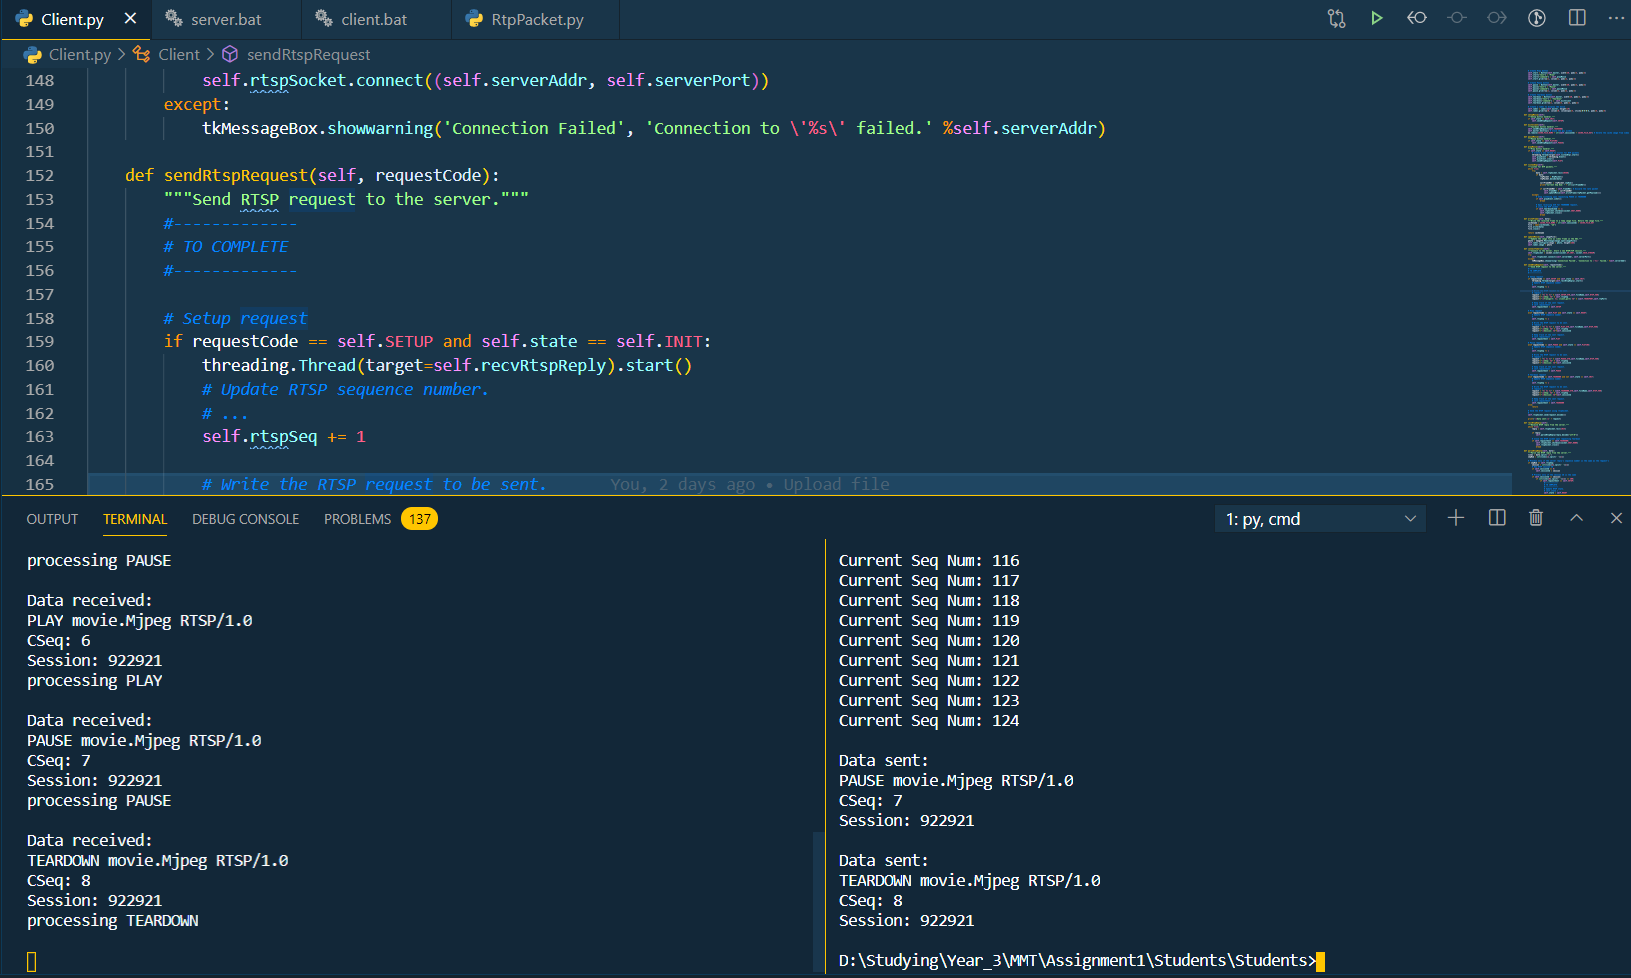
\includegraphics[scale=0.5]{h5.png}  \\
Bên phía client sẽ gửi yêu cầu lên server với data gồm có:
\begin{itemize}
\item Command TEARDOWN
\item Tên video
\item Version RTSP
\item RTSP sequence number
\item Session 
\end{itemize}
Bên phía server sẽ nhận được tất cả data mà client gửi và hiện ra trong terminal cùng với dòng thông báo  \textit{processing TEARDOWN}
\end{enumerate}

\section{Đánh giá kết quả}
\begin{itemize}
\item Về cơ bản, nhóm em đã hoàn thành được phần bài làm. Code được các event cho các button PLAY, SETUP, TEARDOWN, PAUSE.
\item Chương trình chạy khá ổn. Không xuất hiện bug trong quá trình chạy. \\ \\
\begin{tabular}{|c|c|c|c|}
\hline 
MSSV&Học và tên & Công việc\\
\hline 
1814205&Nguyễn Phi Thông&Phân tích yêu cầu, function description, user manual, báo cáo \\
\hline 
1814220&Nguyễn Văn Thuần&Extend, user manual\\
\hline
1812369&Lộc Quốc Huy&class diagram\\
\hline
1613289&Lê Văn Thi&Function description\\
\hline
\end{tabular}
\end{itemize}
\end{document}